\documentclass[a4paper,12pt,ngerman]{scrartcl}

% Language
\usepackage{polyglossia}
\setmainlanguage{german}

% Grafiken
\usepackage{graphicx}

% Make \today print in format "NN<st|nd|rd|th> MM YYYY"
\usepackage{isodate}
\origdate

\linespread{1.15}

% Titel anders formatieren mit: Command, Format, Label, Sep, Before-Code
\usepackage{titlesec}
\titleformat{\section}{\sffamily\Large\bfseries}{}{0pt}{}
\titleformat{\subsection}{\sffamily\large\bfseries}{}{0pt}{}

% Own pagestyle (header and footer)
\usepackage{fancyhdr}
\fancyhf{} % Clear header and footer content
\fancyhead[L]{{\small \textsf{WS 14/15, Informationsvisualisierung}}}
\fancyhead[C]{{\small \textsf{Übung 2}}}
\fancyhead[R]{{\small \textsf{\today}}}
\fancyfoot[C]{\thepage}

% Text in quotes
% Usage: \enquote{To be or not to be.}
\usepackage{csquotes}

% Subliminal refinements towards typographical perfection
\usepackage{microtype}

% Footnotes in section
\usepackage[stable]{footmisc}

% Better refs with \cref{}
\usepackage[capitalize,noabbrev]{cleveref}

% Borders
\usepackage[paper=a4paper,left=20mm,right=20mm,top=30mm,bottom=30mm]{geometry}

\usepackage{longtable}

\begin{document}
\pagestyle{fancy} % Activate own pagestyle

\section{Aufgabe 2.1 | Multivariate Daten\footnote{\scriptsize{Die Qualität der Bilder die man zum Thema Visualisierung im Internet findet lässt oft zu wünschen übrig. Weiterhin werden oft Bilder die als \enquote{png} gespeichert werden sollten, als \enquote{jpg/jpeg} angeboten.}}}
In diesem Abschnitt werden Vor- und Nachteile sowie die Qualifikation und Disqualifikation verschiedener Daten für einige Visualisierungstechniken (i.e. Parallel Coordinates, Scatter Plots, Parallel Sets, Star Plot) beschrieben.

\subsection*{Parallel Coordinates}
Die Visualisierungstechnik Parallel Coordinates (geometrische Visualisierungstechnik) verwendet pro Dimension je eine eigene vertikale Linie. Mehrere dieser sind dann parallel mit einigem Abstand anzuordnen. Konkrete Datensätze sind dann quer zu den vertikelen Linien verlaufende Linien. Diese schneiden sich an der konkreten Wertausprägung mit den vertikalen Linien. Ein Beispiel für Parallel Coordinates ist in \Cref{fig:parallel-coordinates} zu sehen.

\textbf{Parallel Coordinates sind besonders gut zum Erkennen von Korrelationen zwischen Variablen.} Eine positive Korrelation äußert sich in horizontalen Linien, eine negative Korrelation in gekreuzten Linien zwischen zwei Dimensionen.

\begin{figure}[ht]
    \centering
    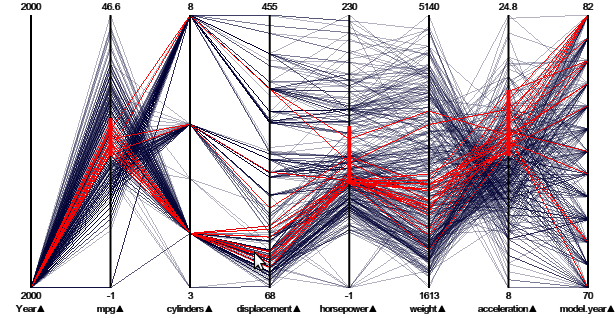
\includegraphics[height=8cm]{includes/parallel-coordinates}
    \caption{Visualisierung mit Hilfe von Parallel Coordinates}
    \label{fig:parallel-coordinates}
\end{figure}

\begin{itemize}
	\item \textbf{Vorteile / Daten die diese Methode qualifizieren:}
	Im Gegensatz zu Scatter Plots auch bei mehr als drei Dimensionen verwendbar. Quantitative (numerische), ordinale und nominale Daten können verwendet werden.

	\item \textbf{Nachteile / Daten die diese Methode disqualifizieren:}
	Bei zu vielen Datenpunkten sollte eingegriffen werden. Als Möglichkeiten sind hier folgende Möglichkeiten anzudenken: Brushing, das Eingrenzen von Wertebereichen, das Vertauschen von Achsen oder verschiedene Clustertechniken wie das hierarchische Clustering.
\end{itemize}

\subsection*{Scatter Plot}
Ein Scatter Plot (geometrische Visualisierungstechnik) beschreibt Datenpunkte, eingetragen in ein 1-,2- oder 3-dimensionales Koordinatensystem --- so wie man es aus der Mathematik kennt. Ein Beispiel für ein Scatter Plot ist in \Cref{fig:scatter-plot} zu sehen.

\textbf{Scatter Plots sind besonders gut zum Erkennen von Objektclustern.} Cluster erkennt man optisch trivial an einer erhöhten Anzahl von Objekten in einem bestimmten Bereich im Koordinatensystem.

\begin{figure}[ht]
    \centering
    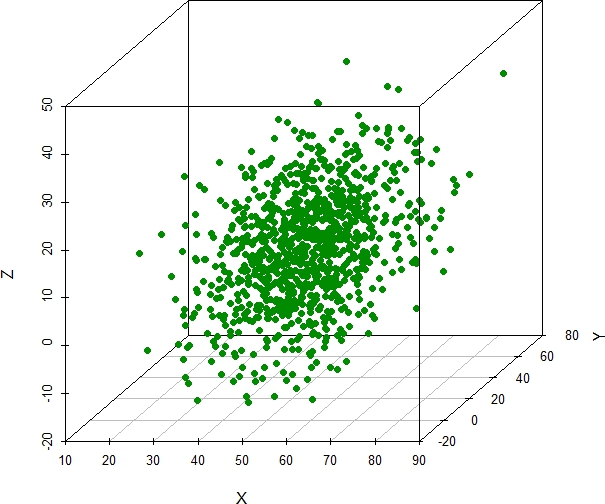
\includegraphics[height=8cm]{includes/scatter-plot}
    \caption{Scatter Plot mit drei Dimensionen}
    \label{fig:scatter-plot}
\end{figure}

\begin{itemize}
	\item \textbf{Vorteile / Daten die diese Methode qualifizieren:}
	Scatter Plots sind gut für eine schnelle Übersicht, zur Strukturfindung und um Zusammenhänge zu erkennen. Daten mit einer, zwei oder maximal drei Dimensionen. Große Anzahl an Datenpunkten möglich. Bei zu vielen Datenpunkten sollten mehrere Datenpunkte zu einem zusammengefasst werden (Diese Eigenschaft haben alle geometrischen Visualisierungstechniken gemeinsam). Quantitative (numerische), ordinale und nominale Daten können verwendet werden.

	\item \textbf{Nachteile / Daten die diese Methode disqualifizieren:}
	Eine hohe Dimensionalität des Datensatzes. Da Scatter Plots in einem kartesischen Koordinatensystem dargestellt werden, können nur 1 und 2 (bzw. begrenzt 3) Dimensionen dargestellt werden. Die dritte Dimension ist vom Betrachtungsmedium abhängig besser (Computer, interaktiv) oder schlechter (Papier, Computer, nicht-interaktiv) interpretierbar.
\end{itemize}

\subsection*{Parallel Sets}
Parallel Sets ist eine geometrische Visualisierungstechnik. Eine horizontale Linie, unterteilt in verschiedene Abschnitte (je nach Ausprägungen der ersten Dimension) wird erstellt. Die verschiedenen Abschnitte gehen nun in unterschiedlicher Breite zur nächsten Dimension über. Am besten erkennt man das ganze an einem Beispiel (\Cref{fig:parallel-sets}). Man erkennt z.B., dass etwa 60\% des harten Wassers (\enquote{hard}) bei einer geringen Temperatur (\enquote{Low}) getrunken wird. Die restlichen 40\% des harten Wassers werden bei hoher Temperatur getrunken (\enquote{High}).

\begin{figure}[ht]
    \centering
    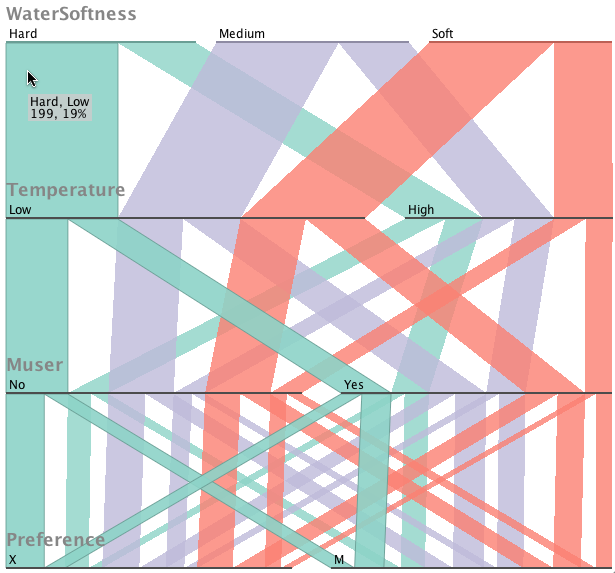
\includegraphics[height=10cm]{includes/parallel-sets}
    \caption{Ein Parallel Set als Beispiel}
    \label{fig:parallel-sets}
\end{figure}

\begin{itemize}
	\item \textbf{Vorteile / Daten die diese Methode qualifizieren:}
	Die Anzahl der möglichen Dimensionen ist theoretisch nicht begrenzt, allerdings verliert die Darstellung an Übersicht wenn zu viele Dimensionen verwendet werden. Auch hier ist es vom Medium abhängig wie gut eine hohe Dimensionsanzahl vom Menschen verarbeitet werden kann. Hovereffekte, die einen bestimmten Teilbaum eines Parallel Sets hervorheben könnten zum Beispiel vom Vorteil sein. Für Parallel Sets können quantitative (numerische), ordinale und nominale Daten verwendet werden.

	\item \textbf{Nachteile / Daten die diese Methode disqualifizieren:}
	Wie in den Vorteilen schon angesprochen wirkt sich eine hohe Dimensionsanzahl negativ auf die Übersichtlichkeit aus.

\end{itemize}

\subsection*{Star Plot}
Der Star Plot (manchmal auch Star Glyph) (icon-basierte Visualisierungstechnik) besteht aus einem Mittelpunkt, einer Linie für jede Datendimension (angeordnet im Kreis) sowie schließlich jeweils eine Linie zwischen den Datendimensionslinien. Somit entsteht eine einem Spinnennetz ähnliche Struktur, ein Polygon. Ein Beispiel (hier mit drei durch Farben getrennte Datensätze) kann in \Cref{fig:star-plot} betrachtet werden.


\textbf{Der Star Plot ist besonders gut zum Erkennen von Ausreißern geeignet.} Das rührt daher, zum einen zwischen Star Plots eine gute Vergleichbarkeit herrscht. Zum anderen stechen Ausreißer durch eine sehr steile Spitze (positiver Ausreißer) oder durch eine fast nicht sichtbare Dimensionsausprägung (negativer Ausreißer) hervor.

\begin{figure}[ht]
    \centering
    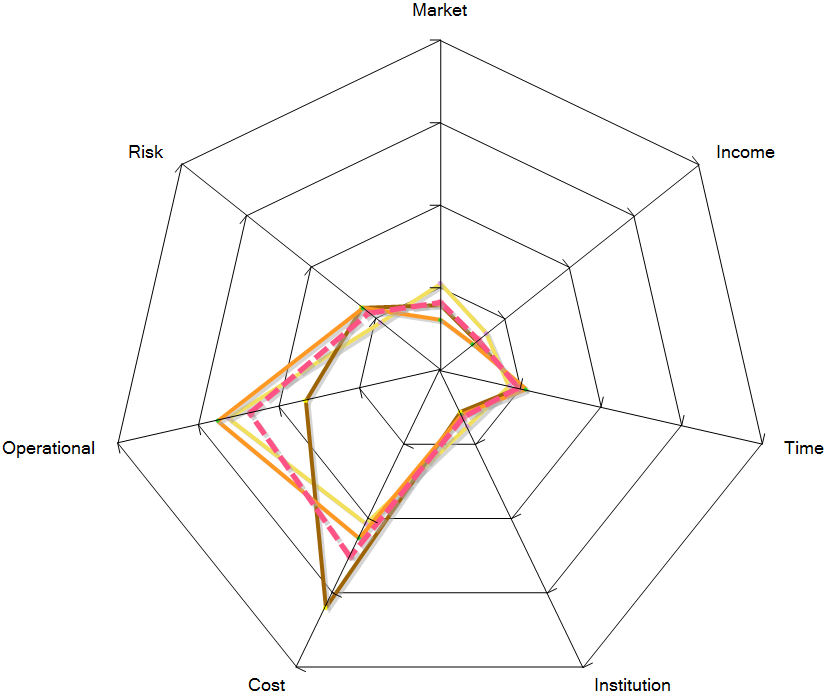
\includegraphics[height=8cm]{includes/star-plot}
    \caption{Ein Parallel Set als Beispiel}
    \label{fig:star-plot}
\end{figure}

\begin{itemize}
	\item \textbf{Vorteile / Daten die diese Methode qualifizieren:}
	Durch die geometrische Anordnung der Ausprägungen ist es schnell möglich, Vergleiche zwischen verschiedenen Datensätzen auszumachen.

	\item \textbf{Nachteile / Daten die diese Methode disqualifizieren:}
	Wie auch bei den geometrischen Visualisierungstechniken ist auch hier die  Skalierbarkeit ein Problem. Existieren viele Dimensionen so ist das Argument der Vergleichbarkeit zwischen verschiedenen Datensätzen nicht mehr gegeben. Weiterhin sind Icon-basierte Visualisierungstechniken, also  auch der Star Plot, nur nützlich wenn qualitative (und nicht quantitative) Aspekte von Datensätzen dargestellt werden sollen. Das kommt daher, dass pro Dimension effektiv nur eine sehr geringe Anzahl an Ausprägungen übersichtlich dargestellt werden kann.

\end{itemize}

\section{Aufgabe 2.2 | RadViz}
\emph{RadViz} (\emph{Radial Coordinates Visualization}) ist eine Visualisierungstechnik, mithilfe derer multivariate Daten innerhalb einer Kreisfläche dargestellt werden. Dazu werden die Variablen durch Punkte auf der Kreislinie repräsentiert. Ein Datum wird im Gegensatz zur Visualisierungstechnik der parallelen Koordinaten nur mittels eines einzigen Punktes visualisiert. Seine Lage im Kreis ergibt sich aus den jeweiligen Variablenwerten, nämlich dort wo nach dem Hooke'schen Gesetz die Summe der verschiedenen Kräfte gleich Null ist. Unter Kraft versteht man hier eine Art Anziehungskraft der Variablen-Repräsentanten, die umso stärker ist, je höher der entsprechende Variablenwert ist. So können auf den ersten Blick Erkenntnisse über eine größere Anzahl von Daten getroffen werden, ohne die einzelnen Variablenwerte vergleichen zu müssen.

\begin{longtable} {| p{0.3\textwidth} | p{0.3\textwidth} | p{0.3\textwidth} |}
Vergleich & Parallel Coordinates & RadViz \\ \hline
\endfirsthead
 & Parallel Coordinates & RadViz\\  \hline
\endhead
Wie leicht verständlich sind die Visualisierungstechniken? & keine Erklärung nötig & es muss zunächst verstanden werden, wie die Punkte im Kreis angeordnet werden\\ \hline
Wie schnell sind Erkenntnisse zu gewinnen? & ohne Hilfsmittel (Einfärben o.Ä.) relativ mühsames Finden von Mustern & sofortige Erkenntnis von Verteilungen\\ \hline
Für welche Datensätze (Art und Größe) eignen sie sich? & sollte verwendet werde, wenn die Einzelwerte der Dimensionen von Bedeutung sind, nur so viele Dimensionen wie Achsen in der Breite wahrnehmbar sind (schätzungsweise $\sim$ 7) & kein Interesse an einzelnen Werten, mehr Dimensionen darstellbar durch Verteilung auf Kreislinie, eignet sich, wenn Variablen unter einem gemeinsamen Aspekt betrachtet werden können und sich im Normalfall gegenseitig beeinflussen \\ \hline
Können sie erweitert werden um zusätzliche Daten darzustellen? & mehr Daten: mehr Linien, höhere Grafik, Gruppieren von Datensätzen & mehr Daten: mehr Punkte, evtl. Gruppieren von Punkten \\
& mehr Dimensionen: breitere Grafik (begrenzt) & mehr Dimensionen: mehr Unterteilungen auf der Kreislinie (schätzungsweise $\sim$ 32 und mehr), Gruppieren von Variablen, dabei evtl. Verlust von Ergebnissen der Visualisierung\\ \hline
Welche Interaktionsmöglichkeiten (Brushing, Einfärben etc) lassen sich mit den Visualisierungen
verknüpfen? & Brushing zur Hervorhebung bestimmter Datensätze, Clustering zur Reduzierung der Komplexität & Brushing nicht möglich, da keine Informationen über Einzelwerte mehr darstellbar sind, Clustering möglich, aber evtl. Verschleiern von Zusammenhängen \\ \hline
Was ist beim Erstellen von Visualisierungen zu bedenken? & sehr begrenzte Anzahl Dimensionen darstellbar, Auswahl der Variablen und Reihenfolge spielen eine Rolle, aber auch bei \enquote{schlechter} Wahl sind Korrelationen zu erkennen & Auswahl der Variablen und deren Anordnung, bei ungünstiger Reihenfolge der Variablen auf der Kreislinie eventuell gar keine Erkenntnisse\\ \hline
Welche Vorteile bieten die Visualisierungen? & alle Einzelwerte werden sichtbar, die Grafik kann nach ersten Erkenntnissen Schritt für Schritt weiter verbessert werden & schnelle Erkenntnisse, gut einsetzbar zur Klassifizierung unbekannter Daten\\ \hline
\end{longtable}

\end{document}
